%@TheDoctorRAB
%
%%%%%
%
%REFERENCES
%neup.bst - numbered citations in order of appearance, short author list with et al in reference section
%nsf.bst - numbered citations in order of appearance, full author list in references section
%standard.bst - citations with author last name with et al for more than 2 authors; full author list in references section
%ans.bst is for ANS only. 
%
%author = {Lastname, Firstname and Lastname, Firstname and Lastname, Firstname} for all bst formats
%bst renders the author list itself
%
%author = {{Nuclear Regulatory Commission}} if the author is an organization, institution, etc., and not people
%
%title = {{}} for all
%
%for all - use \citep{-} - [1] or (Borrelli, 2021) in the text
%standard.bst \cite{-} - Borrelli (2021) in the text
%standard.bst lists references alphabetically
%the rest list numerically
%
%%%%%
\documentclass[11pt,a4paper]{article}
\usepackage[lmargin=1in,rmargin=1in,tmargin=1in,bmargin=1in]{geometry}
\usepackage[pagewise]{lineno} %line numbering
\usepackage{setspace}
\usepackage{ulem} %strikethrough - do not \sout{\cite{}}
\usepackage[pdftex,dvipsnames]{xcolor,colortbl} %change font color
\usepackage{graphicx}
\usepackage{filecontents}
\usepackage{tablefootnote}
\usepackage{footnotehyper}
%\usepackage{subfig}
\usepackage[yyyymmdd]{datetime} %date format
\renewcommand{\dateseparator}{.}
\graphicspath{{../img/}} %path to graphics
\setcounter{secnumdepth}{5} %set subsection to nth level

%fonts
\usepackage{times}
%arial - uncomment next two lines
%\usepackage{helvet}
%\renewcommand{\familydefault}{\sfdefault}

\usepackage{tabto} %general tabbed spacing
\usepackage{longtable} %need to put label at top under caption then \\ - use spacing
\usepackage[stable,hang,flushmargin]{footmisc} %footnotes in section titles and no indent; standard.bst
\usepackage[round,semicolon]{natbib} %use 'numbers' for numbered citations; 'round' for () instead [] for inline citations
%\usepackage[numbers,sort&compress]{natbib} %use 'numbers' for numbered citations; 'round' for () instead [] for inline citations; nsf.bst
\usepackage{enumitem}
\usepackage{boldline}
\usepackage{makecell}
\usepackage{booktabs}
\usepackage{amssymb}
\usepackage{amsmath}
\usepackage{physics}
\usepackage{tabularx}
\usepackage{multirow}
\usepackage{lscape}
\usepackage{array}
\usepackage{caption}
\usepackage{subcaption}
\usepackage[labelfont=bf]{caption}
\usepackage{chngcntr}
\usepackage{hyperref}
\usepackage{sectsty}
\usepackage{textcomp}
\usepackage{lastpage}
\usepackage{xargs} %for \newcommandx
\usepackage[colorinlistoftodos,prependcaption,textsize=small]{todonotes} %makes colored boxes for commenting
\usepackage[toc,title]{appendix}
\usepackage[figure,table]{totalcount}
\usepackage[acronym,nomain,nonumberlist]{glossaries}
\makenoidxglossaries

\usepackage{titlesec}
\titlelabel{\thetitle.\quad}

\usepackage[singlelinecheck=false]{caption}
\captionsetup[table]{skip=7pt,labelformat={default},labelsep=period} %sets a space after table caption
\captionsetup[figure]{skip=7pt,labelformat={default},labelsep=period} %sets space above caption, 'figure' format

\usepackage{wrapfig}
\setlength{\intextsep}{0.20mm}
\setlength{\columnsep}{0.20mm}

%\usepackage{xr} %for revisions - will cross reference from one file to here
%\externaldocument{/path/to/auxfilename} %aux file needed

\newcommand{\edit}[1]{\textcolor{blue}{#1}} %shortcut for changing font color on revised text
\newcommand{\fn}[1]{\footnote{#1}} %shortcut for footnote tag
\newcommand*\sq{\mathbin{\vcenter{\hbox{\rule{.3ex}{.3ex}}}}} %makes a small square as a separator $\sq$
\newcommand{\sk}[1]{\sout{#1}} %shortcut for strikethrough
\newcommand{\x}{\cellcolor{lightgray}} %use to shade in table cell

\newcommand{\acf}{\acrfull} %full acronym
\newcommand{\acl}{\acrlong} %long acronym
\newcommand{\acs}{\acrshort} %short acronym

\newcommand{\acfp}{\acrfullpl} %full acronym plural
\newcommand{\aclp}{\acrlongpl} %long acronym plural
\newcommand{\acsp}{\acrshortpl} %short acronym plural

\newcommandx{\que}[2][1=]{\todo[linecolor=red,backgroundcolor=red!25,bordercolor=red,#1]{#2}} %query
\newcommandx{\sug}[2][1=]{\todo[linecolor=blue,backgroundcolor=blue!25,bordercolor=blue,#1]{#2}} %suggested change
\newcommandx{\cmt}[2][1=]{\todo[linecolor=OliveGreen,backgroundcolor=OliveGreen!25,bordercolor=OliveGreen,#1]{#2}} %comment
\newcommandx{\omt}[2][1=]{\todo[linecolor=Plum,backgroundcolor=Plum!25,bordercolor=Plum,#1]{#2}} %omit

\newcolumntype{L}[1]{>{\raggedright\let\newline\\\arraybackslash\hspace{0pt}}p{#1}} %uses \raggedright with p{} in table column

\makeatletter
\renewcommand\tableofcontents{%
    \@starttoc{toc}%
}
\makeatother

\makeatletter
\renewcommand\listoffigures{%
    \@starttoc{lof}%
}
\makeatother

\makeatletter
\renewcommand\listoftables{%
    \@starttoc{lot}%
}
\makeatother

\makeatletter
\newcommand*\ftp{\fontsize{16.5}{17.5}\selectfont}
\makeatother

%\makeatletter
%\renewcommand\section{%
%    \@startsection{section}{1}{\z@ }{0.50\baselineskip}{0.25\baselineskip}
%    {\normalfont \normalsize \bfseries}}%

%\makeatletter
%\renewcommand\paragraph{%
%    \@startsection{paragraph}{4}{\z@ }{0.25\baselineskip}{-1em}
%    {\normalfont \normalsize \bfseries}}%

%\makeatletter
%\renewcommand\subparagraph{%
%    \@startsection{subparagraph}{5}{\z@ }{0.20\baselineskip}{-1em}
%    {\normalfont \normalsize \itshape }}%

%\makeatletter
%\renewcommand\subsection{%
%    \@startsection{subsection}{2}{\z@ }{0.45\baselineskip}{0.25\baselineskip}
%    { \large \normalsize \bfseries}}%
    
%\setlength{\bibsep}{0pt} %sets space between references
%\renewcommand{\bibsection}{} %suppresses large 'references' heading
%\renewcommand\bibpreamble{\vspace{-0.30\baselineskip}} %sets spacing after heading if not using default references heading

\usepackage{fancyhdr}
\pagestyle{fancy}
\fancyhf{} %move page number to bottom right
\renewcommand{\headrulewidth}{0.5pt} %turn off line in header
\lhead{\scriptsize F. Lastname}
\chead{\scriptsize \textit{NE450 Project 2 - Nuclear engineering basics}}
\rhead{\scriptsize \today}
\rfoot{\thepage}

\begin{filecontents}{references.bib}
    @misc{
        nye15a,
        author = {Nye, Jr., Joseph S.},
        title = {{The World Needs an Arms-control Treaty for Cybersecurity}},
        year = {2015},
        note = {{The Washington Post}}
    }
    @article{
        mil20a,
        author = {Miller, James N.},
        title = {No to no first use — for now},
        journal = {Bulletin of the Atomic Scientists},
        volume = {76},
        pages = {8},
        year  = {2020}
    }
    @incollection{
        mil17a,
        author = {Miller, Steven E.},
        title = {{Cyber Threats, Nuclear Analogies? Divergent Trajectories in Adapting to New Dual-Use Technologies}},
        booktitle = {Understanding Cyber Conflict: 14 Analogies},
        publisher = {Georgetown University Press},
        year = {2017},
        editor = {Perkovich, George and Levite, Ariel E.},
        pages = {161}
    }
    @conference{
        ben20a,
        author = {Benjamin, Jacob and Haney, Michael},
        title = {{Nonproliferation of Cyber Weapons}},
        year = { 2020},
        organization = {Symposium on Cyber Warfare, Cyber Defense, \& Cyber Security },
        address = {Las Vegas, Nevada}
    }
\end{filecontents}

%\newacronym{nrc}{NRC}{United States Nuclear Regulatory Commission}
%\newacronym{}{}{}

\begin{document}

\begin{titlepage}
    \title{
        NE450 - Principles of nuclear engineering\\
        Project 2 - Interaction of radiation with matter\\
    }
    \author{
        Name
        \\ \\ \\
        University of Idaho $\sq$ Idaho Falls Center for Higher Education
        \\ \\
        Nuclear Engineering and Industrial Management Department
        \\ \\ \\
        email 
    }
\clearpage %not have page number on title page
\maketitle
\vspace*{\fill}
\begin{flushright}{
        Total - 200
}
\end{flushright}
\thispagestyle{empty} %start with page number 1 on second page
\end{titlepage}

\printnoidxglossary

\newpage

\section{Elastic scattering}
\paragraph*{(20)}
Derive the elastic scattering energy equation for neutrons.





\newpage

\section{Maxima and minima energies}
\paragraph*{(10)}
Based on this, derive the minimum and maximum scattered neutron energies.





\newpage

\section{Average energy}
\paragraph*{(10)}
Derive the average energy of the scattered neutron and the average energy loss.





\newpage

\section{Mass limit}
\paragraph*{(10)}
Find the limit of $\alpha$ with increasing $A$. What are the implications?





\newpage

\section{Fractional energy loss limit}
\paragraph*{(10)}
Do the same for average fractional energy loss versus $\alpha$.





\newpage

\section{Materials analysis}
\paragraph*{(10)}
Based on this, what materials are more attractive for slowing down neutrons and why?





\newpage


\section{Lethargy functional behavior}
\paragraph*{(10)}
Plot $\xi$ versus $A$. What are the major observations and implications?





\newpage

\section{Lethargy derivation}
\paragraph*{(20)}
Derive $\xi$. Apply the definition of \href{https://courses.lumenlearning.com/uidaho-riskassessment/chapter/statistical-moments/}{expected value for a continuous random variable} and the probability distribution per unit energy loss. \textit{The probability distribution can just be looked up and not derived, but please explain the functional behavior.}





\newpage

\section{Materials functional behavior on collisions}
\paragraph*{(10)}
Plot the average number of collisions versus $A$ for a 2 MeV neutron slowing down to 0.025 eV, for water, boron, carbon, sodium, and uranium. Comment on the results.





\newpage

\section{Inelastic scattering}
\paragraph*{(10)}
Is an inelastic scattering endothermic or exothermic? Please explain why. Similarly, is radiative capture endothermic or exothermic? \textit{Show with math.}





\newpage

\section{Materials for neutron capture}
\paragraph*{(15)}
Why is boron an attractive neutron capture material?





\newpage

\section{Mean free path}
\paragraph*{(15)}
Compute and plot the mean free path for scattering and absorption versus mass for water, boron, carbon, sodium, and uranium and comment on the results. How does this compare to (9)?





\newpage

\section{Maxwell - Most probable energy and velocity}
\paragraph*{(10)}
Derive and compute the most probable energy and velocity for thermal ($1/v$) neutrons.





\newpage

\section{Maxwell - Mean energy and velocity}
\paragraph*{(10)}
Derive and compute mean energy and velocity of thermal ($1/v$) neutrons.





\newpage

\section{Shielding analysis}
\paragraph*{(30)}
Consider two Ar filled rooms of 10 m wide ($x$) by 20 m long ($y$). A neutron source is located at the midpoint of the eastern room. A concrete wall of $x$ thickness separates the two rooms. How thick should the wall be to reduce the flux at the detector on the far western wall to 1\%? What would be the thicknesses for a lead-lined, concrete wall? Roughly compare the costs for each shielding material by deriving a cost function. Consider only scattering and absorption. \textit{See Figures \ref{fig-concrete-wall} and \ref{fig-concrete-lead-wall}.}





\newpage

\section*{Tables}

{%
\let\oldnumberline\numberline%
\renewcommand{\numberline}{\tablename~\oldnumberline}%
\listoftables%
}

\newpage
%Put tables here

\newpage

\section*{Figures}

{%
\let\oldnumberline\numberline%
\renewcommand{\numberline}{\figurename~\oldnumberline}%
\listoffigures%
}

\newpage

\begin{figure}[h!]
    \centering
    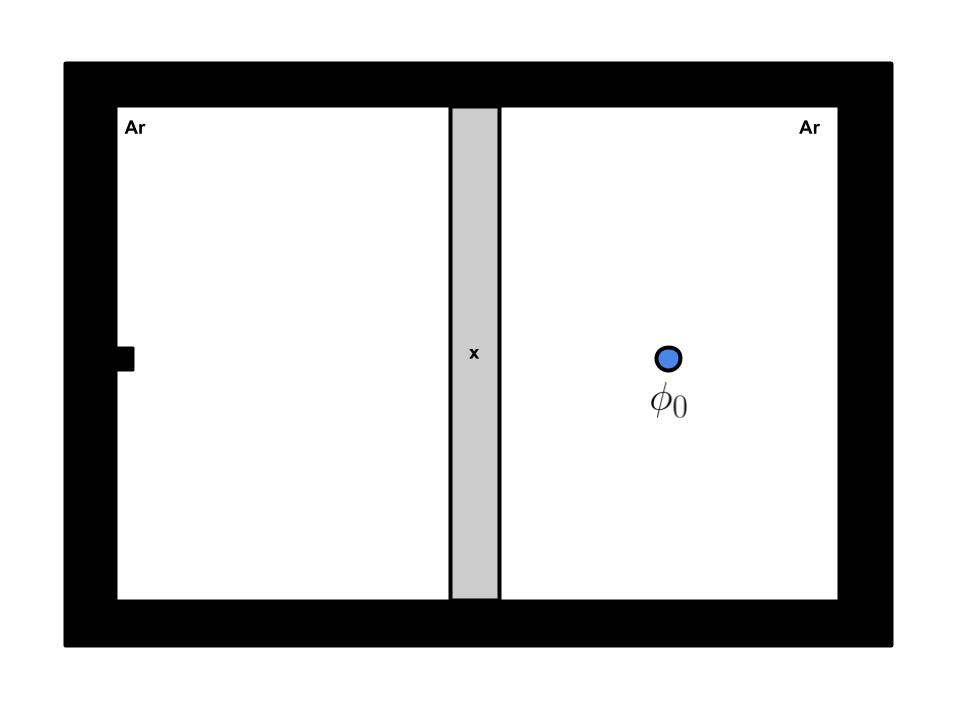
\includegraphics[width=0.75\textwidth]{hw2-15a.jpg}
    \caption{Concrete wall}
    \label{fig-concrete-wall}
\end{figure}

\begin{figure}[h!]
    \centering
    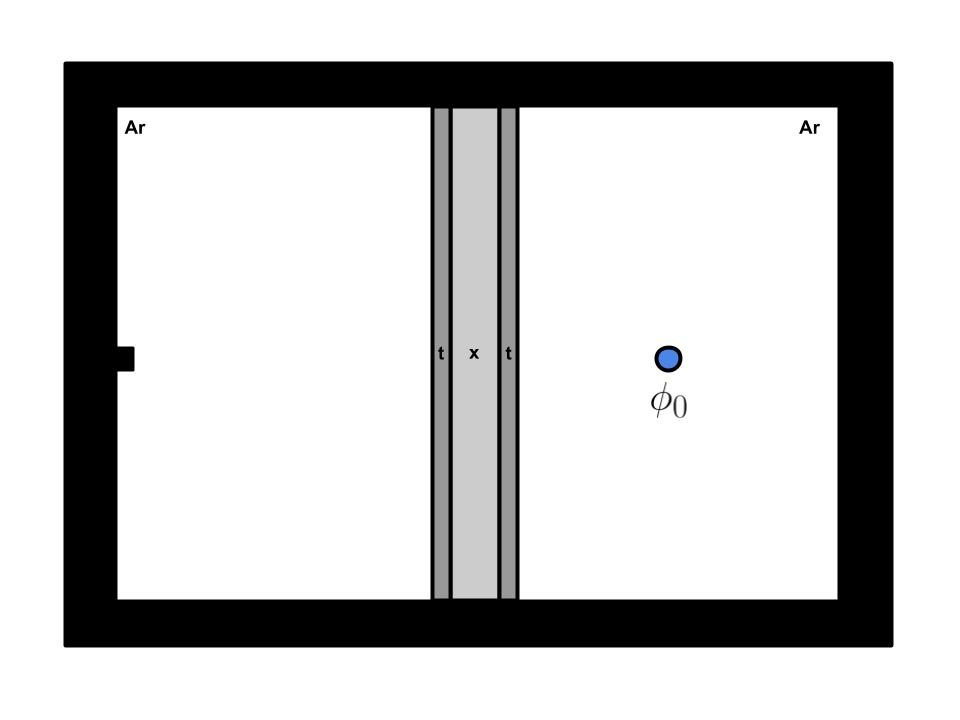
\includegraphics[width=0.75\textwidth]{hw2-15b.jpg}
    \caption{Lead-lined concrete wall}
    \label{fig-concrete-lead-wall}
\end{figure}

\newpage
%Put figures here

\newpage 

%appendix - uncomment below to add - do not uncomment this line

%\begin{appendices}

%\renewcommand{\thesection}{\Roman{section}}

%\section{Just appendix title} \label{}

%\end{appendices}

%\newpage 

\bibliographystyle{nsf}
\setlength{\bibhang}{0pt}
\bibliography{references}

\end{document}
